\documentclass{article}

\usepackage{fancyhdr}
\usepackage{extramarks}
\usepackage{amsmath}
\usepackage{amsthm}
\usepackage{amsfonts}
\usepackage{tikz}
\usepackage[plain]{algorithm}
\usepackage{algpseudocode}
\usepackage{enumerate}
\usepackage{tikz}
\usepackage{dsfont}

\usetikzlibrary{automata,positioning}

%
% Basic Document Settings
%

\topmargin=-0.45in
\evensidemargin=0in
\oddsidemargin=0in
\textwidth=6.5in
\textheight=9.0in
\headsep=0.25in

\linespread{1.1}

\pagestyle{fancy}
\lhead{\hmwkAuthorName}
\chead{\hmwkClass : \hmwkTitle}
\rhead{\firstxmark}
\lfoot{\lastxmark}
\cfoot{\thepage}

\renewcommand\headrulewidth{0.4pt}
\renewcommand\footrulewidth{0.4pt}

\setlength\parindent{0pt}

%
% Create Problem Sections
%

\newcommand{\enterProblemHeader}[1]{
    \nobreak\extramarks{}{Problem \arabic{#1} continued on next page\ldots}\nobreak{}
    \nobreak\extramarks{Problem \arabic{#1} (continued)}{Problem \arabic{#1} continued on next page\ldots}\nobreak{}
}

\newcommand{\exitProblemHeader}[1]{
    \nobreak\extramarks{Problem \arabic{#1} (continued)}{Problem \arabic{#1} continued on next page\ldots}\nobreak{}
    \stepcounter{#1}
    \nobreak\extramarks{Problem \arabic{#1}}{}\nobreak{}
}

\newcommand*\circled[1]{\tikz[baseline=(char.base)]{
		\node[shape=circle,draw,inner sep=2pt] (char) {#1};}}


\setcounter{secnumdepth}{0}
\newcounter{partCounter}
\newcounter{homeworkProblemCounter}
\setcounter{homeworkProblemCounter}{1}
\nobreak\extramarks{Problem \arabic{homeworkProblemCounter}}{}\nobreak{}

%
% Homework Problem Environment
%
% This environment takes an optional argument. When given, it will adjust the
% problem counter. This is useful for when the problems given for your
% assignment aren't sequential. See the last 3 problems of this template for an
% example.
%

\newenvironment{homeworkProblem}[1][-1]{
    \ifnum#1>0
        \setcounter{homeworkProblemCounter}{#1}
    \fi
    \section{Problem \arabic{homeworkProblemCounter}}
    \setcounter{partCounter}{1}
    \enterProblemHeader{homeworkProblemCounter}
}{
    \exitProblemHeader{homeworkProblemCounter}
}

%
% Homework Details
%   - Title
%   - Class
%   - Due date
%   - Name
%   - Student ID

\newcommand{\hmwkTitle}{Homework\ \#01}
% \newcommand{\hmwkTitle}{Homework\\ \circled{1}}
\newcommand{\hmwkClass}{SI252 Reinforcement Learning}
\newcommand{\hmwkDueDate}{March 9, 2025}
\newcommand{\hmwkAuthorName}{Zhou Shouchen}
\newcommand{\hmwkAuthorID}{2021533042}


%
% Title Page
%

\title{
    \vspace{2in}
    \textmd{\textbf{\hmwkClass:\\  \hmwkTitle}} \\
    \normalsize\vspace{0.1in}\small{Due\ on\ \hmwkDueDate\ at 11:59 a.m.(CST)} \\
	\vspace{4in}
}

\author{
	Name: \textbf{\hmwkAuthorName} \\
	Student ID: \hmwkAuthorID}
\date{}

\renewcommand{\part}[1]{\textbf{\large Part \Alph{partCounter}}\stepcounter{partCounter}\\}

%
% Various Helper Commands
%

% Useful for algorithms
\newcommand{\alg}[1]{\textsc{\bfseries \footnotesize #1}}
% For derivatives
\newcommand{\deriv}[1]{\dfrac{\mathrm{d}}{\mathrm{d}x} (#1)}
% For partial derivatives
\newcommand{\pderiv}[2]{\dfrac{\partial}{\partial #1} (#2)}
% Integral dx
\newcommand{\dx}{\mathrm{d}x}
\newcommand{\du}{\mathrm{d}u}
\newcommand{\dr}{\mathrm{d}r}
\newcommand{\dS}{\mathrm{d}S}
\newcommand{\dtheta}{\mathrm{d}\theta}
\newcommand{\dphi}{\mathrm{d}\phi}

% Alias for the Solution section header
\newcommand{\solution}{\textcolor{blue}{\textbf{\large Solution}} \\}
% Probability commands: Expectation, Variance, Covariance, Bias
\newcommand{\E}{\mathbb{E}}
\newcommand{\Var}{\mathrm{Var}}
\newcommand{\Cov}{\mathrm{Cov}}
\newcommand{\Bias}{\mathrm{Bias}}
\newcommand{\Unif}{\operatorname{Unif}}
\newcommand{\Beta}{\operatorname{Beta}}
\newcommand{\Bin}{\operatorname{Bin}}
\newcommand{\N}{\mathcal{N}}
\newcommand{\I}{\mathds{1}}


\begin{document}

\maketitle
\pagebreak

\begin{homeworkProblem}

[BH Chapter 11, Problem 2]. Let $X_0, X_1, X_2 \ldots$ be an irreducible Markov chain with state space $\{1,2, \ldots, M\}$. $M \geq 3$, transition matrix $Q=\left(q_{i,j}\right)$, and stationary distribution $\mathbf{s}=\left(s_1, \ldots, s_M\right)$. Let the initial state $X_0$ follow the stationary distribution, i.e., $P\left(X_0=i\right)=s_i$.

(a) On average, how many of $X_0, X_1, \ldots, X_9$ equal 3? (In terms of $\mathbf{s}$; simplify.)

(b) Let $Y_n=\left(X_n-1\right)\left(X_n-2\right)$. For $M=3$, find an example of $Q$ (the transition matrix for the \textit{original} chain $X_0, X_1, \ldots$ ) where $Y_0, Y_1, \ldots$ is Markov, and another example of $Q$ where $Y_0, Y_1, \ldots$ is not Markov. In your examples, make $q_{i,i}>0$ for at least one $i$ and make sure it is possible to get from any state to any other state eventually.

\solution

(a) Let the indicator $\I_i$ donate wheher $X_i=3$, and $N$ be the number of $X_0,\ldots,X_9$ equal to 3. Since the initial state $X_0$ follows the stationary distribution, so $X_1,\ldots,X_9$ also follow the stationary distribution. i.e.
$$P(X_i=3)=s_3, \forall i\in\{0,\ldots,9\}$$
Then we can get that:
$$\E[N] = \E\left[\sum_{i=0}^9 \I_i\right] = \sum_{i=0}^9 \E\left[\I_i\right] = \sum_{i=0}^9 P(X_i=3) = \sum_{i=0}^9 s_3 = 10s_3$$

(b) Since $M=3$, and the relationship between $X_i$ and $Y_i$ is:
\begin{align*}
X_i=1 &\Rightarrow Y_i=0 \\
X_i=2 &\Rightarrow Y_i=0 \\
X_i=3 &\Rightarrow Y_i=2
\end{align*}
Define $g(y)$ be a set of values of $x$ such that $Y=g(X)$. i.e. $g(0)=\{1,2\}, g(2)=\{3\}$.

To let $Y_0,Y_1,\ldots$ be Markov, we need to make sure that
$$P(Y_{n+1}=y_{n+1}|Y_n=y_n,\ldots,Y_0=y_0) = P(Y_{n+1}=y_{n+1}|Y_n=y_n)$$
Since $Y_i$ have $2$ possible values, so we can discuss them in $4$ cases:
\begin{itemize}
\item $Y_{n+1}=2$, $Y_n=2$:
\begin{align*}
&\quad\ P(Y_{n+1}=2|Y_n=2,Y_{n-1}=y_{n-1},\ldots,Y_0=y_0) \\
&= P(X_{n+1}=3|X_n=3,X_{n-1}=x_{n-1},\ldots,X_0=x_0) \\
&= P(X_{n+1}=3|X_n=3) \\
&= P(Y_{n+1}=2|Y_n=2)
\end{align*}

\item $Y_{n+1}=0$, $Y_n=2$:
\begin{align*}
&\quad\ P(Y_{n+1}=0|Y_n=2,Y_{n-1}=y_{n-1},\ldots,Y_0=y_0) \\
&= P(X_{n+1}\in g(0)|X_n=3,X_{n-1}=x_{n-1},\ldots,X_0=x_0) \\
&= P(X_{n+1}=1|X_n=3,X_{n-1}=x_{n-1},\ldots,X_0=x_0) + P(X_{n+1}=2|X_n=3,X_{n-1}=x_{n-1},\ldots,X_0=x_0) \\
&= P(X_{n+1}=1|X_n=3) + P(X_{n+1}=2|X_n=3) \\
&= P(X_{n+1}\in g(0)|X_n=3) \\
&= P(Y_{n+1}=0|Y_n=2)
\end{align*}

\item $Y_{n+1}=2$, $Y_n=0$, combined with LOTP:
\begin{align*}
&\quad\ P(Y_{n+1}=2|Y_n=0,Y_{n-1}=y_{n-1},\ldots,Y_0=y_0) \\
&= \sum_{x_n=1,2} P(X_{n+1}=3|X_n=x_n,X_n\in g(0),\ldots,X_0\in g(y_0))P(X_n=x_n|X_n\in g(0),\ldots,X_0\in g(y_0)) \\
&= \sum_{x_n=1,2} P(X_{n+1}=3|X_n=x_n)P(X_n=x_n|X_n\in g(0),\ldots,X_0\in g(y_0))
\end{align*}
Let $\alpha_1=P(X_n=1|X_n\in g(0),\ldots,X_0\in g(y_0)),\alpha_2=P(X_n=2|X_n\in g(0),\ldots,X_0\in g(y_0))$. So we have
\begin{align*}
\alpha_1+\alpha_2 &= 1 \\
P(Y_{n+1}=2|Y_n=0,Y_{n-1}=y_{n-1},\ldots,Y_0=y_0) &= \alpha_1q_{1,3}+\alpha_2q_{2,3}
\end{align*}
Since $g(0)$ have $2$ elements, so there exists many combinations to make $\alpha_1,\alpha_2$ take different values, but $\alpha_1+\alpha_2$ always holds. However, to make the Markov property holds, we need to make sure that $\alpha_1q_{1,3}+\alpha_2q_{2,3}=P(Y_{n+1}=2|Y_n=0)$, where $P(Y_{n+1}=2|Y_n=0),q_{2,3}$ are constants. Thus it must have
$$\alpha_1(q_{1,3}-q_{2,3})=P(Y_{n+1}=2|Y_n=0)-q_{2,3} \Rightarrow q_{1,3}=q_{2,3}$$

\item $Y_{n+1}=0$, $Y_n=0$, combined with LOTP:
\begin{align*}
&\quad\ P(Y_{n+1}=0|Y_n=0,Y_{n-1}=y_{n-1},\ldots,Y_0=y_0) \\
&= \sum_{x_n=1,2} P(X_{n+1}\in g(0)|X_n=x_n,X_n\in g(0),\ldots,X_0\in g(y_0))P(X_n=x_n|X_n\in g(0),\ldots,X_0\in g(y_0)) \\
&= \sum_{x_n=1,2} P(X_{n+1}\in g(0)|X_n=x_n)P(X_n=x_n|X_n\in g(0),\ldots,X_0\in g(y_0))
\end{align*}
Let $\alpha_1'=P(X_n=1|X_n\in g(0),\ldots,X_0\in g(y_0)),\alpha_2'=P(X_n=2|X_n\in g(0),\ldots,X_0\in g(y_0))$. So we have
\begin{align*}
\alpha_1'+\alpha_2' &= 1 \\
P(Y_{n+1}=0|Y_n=0,Y_{n-1}=y_{n-1},\ldots,Y_0=y_0) &= \alpha_1'\left(q_{1,1}+q_{1,2}\right)+\alpha_2'\left(q_{2,1}+q_{2,2}\right)
\end{align*}
Similarly to the analysis above, to make the Markov property holds, it has
$$q_{1,1}+q_{1,2}=q_{2,1}+q_{2,2}$$
So above all, if $q_{1,3}=q_{2,3}$ and $q_{1,1}+q_{1,2}=q_{2,1}+q_{2,2}$, then $Y_0,Y_1,\ldots$ is Markov. \\
And example of $Q$ where $Y_0,Y_1,\ldots$ is Markov is:
$$Q=\begin{pmatrix}
\frac{1}{3} & \frac{1}{3} & \frac{1}{3} \\
\frac{1}{3} & \frac{1}{3} & \frac{1}{3} \\
\frac{1}{3} & \frac{1}{3} & \frac{1}{3}
\end{pmatrix}$$
Examplt of $Q$ where $Y_0,Y_1,\ldots$ is not Markov is:
$$Q=\begin{pmatrix}
\frac{1}{2} & \frac{1}{2} & 0 \\
\frac{1}{3} & \frac{1}{3} & \frac{1}{3} \\
\frac{1}{3} & \frac{1}{3} & \frac{1}{3}
\end{pmatrix}$$

\end{itemize}

\end{homeworkProblem}

\newpage
\begin{homeworkProblem}

\textbf{Student MDPs}

(a) Given the equal option policy, reproduce the state values \& state-action values for student MDP with both theoretical method and iterative policy evaluation method. Then discuss the pros and cons of each method.
\begin{figure}[h]
    \centering
    \includegraphics[width=0.5\textwidth]{./figure/MDP1.png}
\end{figure}

(b) Reproduce the optimal state values, optimal state-action values, and optimal policy for student MDP with theoretical method, policy iteration method and value iteration method. Then discuss the pros and cons of each method.
\begin{figure}[h]
    \centering
    \includegraphics[width=0.5\textwidth]{./figure/MDP2.png}\
    \vspace{-0.5cm}
\end{figure}

\solution

We can number the states for convience, written on the figure with purple $s_1,\cdots,s_4$(The terminal state is ignored, whose state value and action-state values are all $0$). And the action space is $\A=$\{Facebook, Quit, Study, Sleep, Pub\}. And the rewards and transition probabilities are given in the figure. And the discount factor is $\gamma=1$. The codes for (a), (b) could be found in the `hw5\_code.ipynb' file.

(a) From the Bellman Expectation Equations for MDPs, we can get that
\begin{align*}
v_{\pi}(s) &= \sum_{a \in \A}\pi(a|s)\left(\R_s^a + \gamma \sum_{s' \in \mS} \mP_{s,s'}^a v_{\pi}(s')\right) \\
q_{\pi}(s,a) &= \R_s^a + \gamma \sum_{s' \in \mS} \mP_{s,s'}^a v_{\pi}(s')
\end{align*}
1. Theoretical method: \\
We can use the inplace method to solve the state values $v_{\pi}(s)$, i.e. solve the equations:
\begin{align*}
\qquad&\begin{cases}
v_{\pi}(s_1) = 0.5 * (\R_{s_1}^{\text{Facebook}} + 1 * 1 * v_{\pi}(s_1)) + 0.5 *(\R_{s_1}^{\text{Quit}} + 1 * 1 * v_{\pi}(s_2)) \\
v_{\pi}(s_2) = 0.5 * (\R_{s_2}^{\text{Facebook}} + 1 * 1 * v_{\pi}(s_1)) + 0.5 *(\R_{s_2}^{\text{Study}} + 1 * 1 * v_{\pi}(s_3)) \\
v_{\pi}(s_3) = 0.5 * (\R_{s_3}^{\text{Study}} + 1 * 1 * v_{\pi}(s_4)) + 0.5 *(\R_{s_3}^{\text{Sleep}} + 1 * 1 * 0) \\
v_{\pi}(s_4) = 0.5 * (\R_{s_4}^{\text{Study}} + 1 * 1 * 0) + 0.5 * \left(\R_{s_4}^{\text{Pub}} + 1 * \left(0.2 * v_{\pi}(s_2) + 0.4 * v_{\pi}(s_3) + 0.4 * v_{\pi}(s_4)\right)\right)
\end{cases} \\
\Rightarrow\ &\begin{cases}
v_{\pi}(s_1) - v_{\pi}(s_2) = -1 \\
-v_{\pi}(s_1) + 2v_{\pi}(s_2) - v_{\pi}(s_3) = -3 \\
2v_{\pi}(s_3) - v_{\pi}(s_4) = -2 \\
-v_{\pi}(s_2) - 2v_{\pi}(s_3) + 8v_{\pi}(s_4) = 55
\end{cases} \\
\Rightarrow\ &\begin{cases}
v_{\pi}(s_1) = -2.3076923076923066 \\
v_{\pi}(s_2) = -1.3076923076923066 \\
v_{\pi}(s_3) = 2.6923076923076934 \\
v_{\pi}(s_4) = 7.384615384615385
\end{cases}
\qquad\approx\qquad\begin{cases}
v_{\pi}(s_1) = 2.3 \\
v_{\pi}(s_2) = -1.3 \\
v_{\pi}(s_3) = 2.7 \\
v_{\pi}(s_4) = 7.4
\end{cases}
\end{align*}

With calculated state values, we can get the state-action values:
$$\begin{cases}
q_{\pi}(s_1, \text{Facebook}) &= -3.3076923076923066 \\
q_{\pi}(s_1, \text{Quit}) &= -1.3076923076923066 \\
q_{\pi}(s_2, \text{Facebook}) &= -3.3076923076923066 \\
q_{\pi}(s_2, \text{Study}) &= 0.6923076923076934 \\
q_{\pi}(s_3, \text{Study}) &= 5.384615384615385 \\
q_{\pi}(s_3, \text{Sleep}) &= 0 \\
q_{\pi}(s_4, \text{Study}) &= 10 \\
q_{\pi}(s_4, \text{Pub}) &= 4.76923076923077
\end{cases} \qquad\approx\qquad \begin{cases}
q_{\pi}(s_1, \text{Facebook}) &= -3.3 \\
q_{\pi}(s_1, \text{Quit}) &= -1.3 \\
q_{\pi}(s_2, \text{Facebook}) &= -3.3 \\
q_{\pi}(s_2, \text{Study}) &= 0.7 \\
q_{\pi}(s_3, \text{Study}) &= 5.4 \\
q_{\pi}(s_3, \text{Sleep}) &= 0 \\
q_{\pi}(s_4, \text{Study}) &= 10 \\
q_{\pi}(s_4, \text{Pub}) &= 4.8
\end{cases}$$

2. Iterative Policy Evaluation Method: \\
The threshold is set to be $\epsilon=10^{-3}$, after 26 iterations, the state values convergence, and the results are
$$\begin{cases}
v_{\pi}(s_1) = -2.3116692858874535 \\
v_{\pi}(s_2) = -1.3102871136591983 \\
v_{\pi}(s_3) = 2.6919968668115835 \\
v_{\pi}(s_4) = 7.384101760095685
\end{cases}
\qquad\approx\qquad\begin{cases}
v_{\pi}(s_1) = 2.3 \\
v_{\pi}(s_2) = -1.3 \\
v_{\pi}(s_3) = 2.7 \\
v_{\pi}(s_4) = 7.4
\end{cases}$$
The correspondence state-action values are
$$\begin{cases}
q_{\pi}(s_1, \text{Facebook}) &= -3.3116692858874535 \\
q_{\pi}(s_1, \text{Quit}) &= -1.3102871136591983 \\
q_{\pi}(s_2, \text{Facebook}) &= -3.3116692858874535 \\
q_{\pi}(s_2, \text{Study}) &= 0.6919968668115835 \\
q_{\pi}(s_3, \text{Study}) &= 5.384101760095685 \\
q_{\pi}(s_3, \text{Sleep}) &= 0 \\
q_{\pi}(s_4, \text{Study}) &= 10 \\
q_{\pi}(s_4, \text{Pub}) &= 4.768382028031068
\end{cases} \qquad\approx\qquad \begin{cases}
q_{\pi}(s_1, \text{Facebook}) &= -3.3 \\
q_{\pi}(s_1, \text{Quit}) &= -1.3 \\
q_{\pi}(s_2, \text{Facebook}) &= -3.3 \\
q_{\pi}(s_2, \text{Study}) &= 0.7 \\
q_{\pi}(s_3, \text{Study}) &= 5.4 \\
q_{\pi}(s_3, \text{Sleep}) &= 0 \\
q_{\pi}(s_4, \text{Study}) &= 10 \\
q_{\pi}(s_4, \text{Pub}) &= 4.8
\end{cases}$$

3. Pros and cons: \\
Theoretical method calculates the optimal state values $v_*(s)$ by solving a linear system, and its advantage lies in providing an exact solution in one go. It constructs the matrix $\left(I-\gamma\mP^{\pi}\right)^{-1}\R^{\pi}$ to solve for the optimal state values, avoiding the need for iterative processes. The result is accurate, and when the model is  relatively small in scale, the complexity is relatively low. \\
However, the disadvantage of this method is that getting inverse matrix requires $O(n^3)$ time complexity, where $n$ is the number of states. When the state space and action space are large, the theoretical method may become computationally expensive and inefficient. \\

Iterative policy evaluation method iteratively updates the state value function to approximate the optimal solution. It can gradually converge to the optimal solution it can still effectively perform evaluations when the spaces are large. It may not be the accurate solution, but close to the accurate one and computational friendly. \\
However, its disadvantage is that it may have cases that converges slowly. When chasing for a more accurate solution, i.e. setting $\epsilon$ to be smaller, it may converge much slower. \\

(b) Let $v_*(s)$ be the optimal state value function, and $q_*(s,a)$ be the optimal state-action value function. The Bellman Optimality Equation is:
\begin{align*}
v_*(s) &= \max_{a \in \A}\left(\R_s^a + \gamma \sum_{s' \in \mS} \mP_{s,s'}^a v_*(s')\right) \\
q_*(s,a) &= \R_s^a + \gamma \sum_{s' \in \mS} \mP_{s,s'}^a v_*(s') \\
\pi_*(a|s) &= \begin{cases}
1 & \text{if } a\in \argmax\limits_{a\in\A}q_*(s,a) \\
0 & \text{otherwise}
\end{cases}
\end{align*}
Thus, we could get the optimal state value function $v_*(s)$ with different methods, then get optimal state-action value function $q_*(s,a)$ using $v_*(s)$ and final get the optimal policy $\pi^*(a|s)$ using $q_*(s,a)$.

1. Theoretical method: \\
We can re-write the definition of $v_*(s)$ into the an inequality form:
\begin{align*}
v_*(s) = \max_{a \in \A}\left(\R_s^a + \gamma \sum_{s' \in \mS} \mP_{s,s'}^a v_*(s')\right)
&\Rightarrow v_*(s) \geq \R_s^a + \gamma \sum_{s' \in \mS} \mP_{s,s'}^a v_*(s')\ \ \forall a\in A \\
&\Rightarrow -v_*(s) + \gamma \sum_{s' \in \mS} \mP_{s,s'}^a v_*(s') \leq -\R_s^a\ \ \forall a\in A
\end{align*}
So the Bellman Optimality Equation could be re-written into a set of inequality constrains. As we known of the basic knowledge of convex optimization, the optimal solution must be lying on the inconstraint set for the Linear Programming problem, thus we can add a linear objective function to ensure the inequality constrains try to be equal. So the final LP problem is:
\begin{align*}
\min_{v} &\qquad\quad \sum_{s \in \mS} v(s) \\
\text{s.t.} &\ -v(s) + \gamma \sum_{s' \in \mS} \mP_{s,s'}^a v(s') \leq -\R_s^a\ \ \forall s\in\mS, a\in \A
\end{align*}
Thus, solve the LP problem with optimizers, we can get the theoritical optimal state values, optimal state-action values and optimal policy. The constructed LP is:
\begin{align*}
\min_{v} &\qquad\quad \sum_{s \in \mS} v(s) \\
\text{s.t.} &\ \begin{pmatrix}
0 & 0 & 0 & 0 \\
-1 & 1 & 0 & 0 \\
1 & -1 & 0 & 0 \\
0 & -1 & 1 & 0 \\
0 & 0 & -1 & 0 \\
0 & 0 & -1 & 0 \\
0 & 0.2 & 0.4 & -0.6 \\
0 & 0 & 0 & -1
\end{pmatrix}
\begin{pmatrix}
v(s_1) \\ v(s_2) \\ v(s_3) \\ v(s_4)
\end{pmatrix} \leq \begin{pmatrix}
1 \\ 0 \\ 1 \\ 2 \\ 0 \\ 2 \\ -1 \\ -10
\end{pmatrix}
\end{align*}
The result is:
$$\begin{cases}
v_*(s_1) = 6 \\
v_*(s_2) = 6 \\
v_*(s_3) = 8 \\
v_*(s_4) = 10
\end{cases} \qquad \Rightarrow \qquad \begin{cases}
q_*(s_1, \text{Facebook}) &= 5 \\
q_*(s_1, \text{Quit}) &= 6 \\
q_*(s_2, \text{Facebook}) &= 5 \\
q_*(s_2, \text{Study}) &= 6 \\
q_*(s_3, \text{Study}) &= 8 \\
q_*(s_3, \text{Sleep}) &= 0 \\
q_*(s_4, \text{Study}) &= 10 \\
q_*(s_4, \text{Pub}) &= 9.4
\end{cases} \qquad \Rightarrow \qquad \begin{cases}
\pi_*(s_1) = \text{Quit} \\
\pi_*(s_2) = \text{Study} \\
\pi_*(s_3) = \text{Study} \\
\pi_*(s_4) = \text{Study}
\end{cases}$$

2. Policy Iteration Method: \\
We can applying policy iteration method through the following pseudocode to get $v_*(s)$ and $\pi_*(s)$, then get $q_*(s,a)$ by Bellman Optimality Equation using $v_*(s)$: \\
\begin{figure}[!htbp]
    \centering
    \vspace{-0.5cm}
    \includegraphics[width=0.55\textwidth]{./figure/policy_iteration_pseudocode}
    \vspace{-0.5cm}
\end{figure}
The result is:
$$\begin{cases}
v_*(s_1) = 6 \\
v_*(s_2) = 6 \\
v_*(s_3) = 8 \\
v_*(s_4) = 10
\end{cases} \qquad \Rightarrow \qquad \begin{cases}
q_*(s_1, \text{Facebook}) &= 5 \\
q_*(s_1, \text{Quit}) &= 6 \\
q_*(s_2, \text{Facebook}) &= 5 \\
q_*(s_2, \text{Study}) &= 6 \\
q_*(s_3, \text{Study}) &= 8 \\
q_*(s_3, \text{Sleep}) &= 0 \\
q_*(s_4, \text{Study}) &= 10 \\
q_*(s_4, \text{Pub}) &= 9.4
\end{cases} \qquad \Rightarrow \qquad \begin{cases}
\pi_*(s_1) = \text{Quit} \\
\pi_*(s_2) = \text{Study} \\
\pi_*(s_3) = \text{Study} \\
\pi_*(s_4) = \text{Study}
\end{cases}$$
It totally run policy iteration 2 times, and the policy evaluation used 24+4=30 iterations.

3. Value Iteration Method: \\
We can applying policy iteration method through the following pseudocode to get $v_*(s)$ and $q_*(s,a)$, then get $\pi_*(s)$ through $q_*(s,a)$:
\begin{figure}[!htbp]
    \centering
    \includegraphics[width=0.7\textwidth]{./figure/value_iteration_pseudocode}
\end{figure}

It totally run value iteration 4 times. The result is:
$$\begin{cases}
v_*(s_1) = 6 \\
v_*(s_2) = 6 \\
v_*(s_3) = 8 \\
v_*(s_4) = 10
\end{cases} \qquad \Rightarrow \qquad \begin{cases}
q_*(s_1, \text{Facebook}) &= 5 \\
q_*(s_1, \text{Quit}) &= 6 \\
q_*(s_2, \text{Facebook}) &= 5 \\
q_*(s_2, \text{Study}) &= 6 \\
q_*(s_3, \text{Study}) &= 8 \\
q_*(s_3, \text{Sleep}) &= 0 \\
q_*(s_4, \text{Study}) &= 10 \\
q_*(s_4, \text{Pub}) &= 9.4
\end{cases} \qquad \Rightarrow \qquad \begin{cases}
\pi_*(s_1) = \text{Quit} \\
\pi_*(s_2) = \text{Study} \\
\pi_*(s_3) = \text{Study} \\
\pi_*(s_4) = \text{Study}
\end{cases}$$

4. Pros and cons: \\
Theoretical method: \\
Advantage: It can get an exact and optimal solution by formulating the Bellman Optimality Equation as a set of linear inequalities, then solving the problem using linear programming. This method guarantees that the resulting state values and policies are optimal because it directly solves the problem mathematically without iteration. It is highly efficient for small-scale problems. \\
Disadvantages: It is not suitable for large-scale problems as solving the optimization problem requires a much more time, which is not efficient. \\

Policy Iteration: \\
Advantage: By alternating between policy evaluation and policy improvement, the optimal policy can be found and the corresponding optimal state value $V_x (s) $can be calculated, resulting in high accuracy for policy evaluation. \\
Disadvantages: Requires repeated strategy evaluation and improvement, slow convergence speed, especially when the state space is large. \\

Value Iteration: \\
Advantage: By continuously updating the state value function, it is possible to directly approximate the optimal state value $V_x (s) $. It is based on greedy selection, calculating the optimal action only at last. \\
Disadvantage: Due to updating the values of all states at each iteration, it may require more iterations to converge when the state space is large.

\end{homeworkProblem}

\newpage
\begin{homeworkProblem}

[BH Chapter 11, Problem 6]. Daenerys has three dragons: Drogon, Rhaegal, and Viserion. Each dragon independently explores the world in search of tasty morsels. Let $X_n, Y_n, Z_n$ be the locations at time $n$ of Drogon, Rhaegal, Viserion respectively, where time is assumed to be discrete and the number of possible locations is a finite number $M$. Their paths $X_0, X_1, X_2 \ldots$; $Y_0, Y_1, Y_2, \ldots ;$ and $Z_0, Z_1, Z_2, \ldots$ are independent Markov chains with the same stationary distribution $\mathbf{s}$. Each dragon starts out at a random location generated according to the stationary distribution.

(a) Let state 0 be home (so $s_0$ is the stationary probability of the home state). Find the expected number of times that Drogon is at home, up to time 24, i.e., the expected number of how many of $X_0, X_1, \ldots, X_{24}$ are state 0 (in terms of $s_0$ ).

(b) If we want to track all 3 dragons simultaneously, we need to consider the vector of positions, $\left(X_n, Y_n, Z_n\right)$. There are $M^3$ possible values for this vector; assume that each is assigned a number from 1 to $M^3$, e.g., if $M=2$ we could encode the statex $(0,0,0),(0,0,1),(0,1,0), \ldots,(1,1,1)$ as $1,2,3, \ldots, 8$ respectively. Let $W_n$ be the number between 1 and $M^3$ representing ($X_n, Y_n, Z_n$). Determine whether $W_0, W_1, \ldots$ is a Markov chain.

(c) Given that all 3 dragons start at home at time 0, find the expected time it will take for all 3 to be at home again at the same time.

\solution

(a) Let the indicator $\I_i$ denote whether $X_i=0$, and $N$ be the number of $X_0,\ldots,X_{24}$ equal to 0. Since the initial state $X_0$ follows the stationary distribution, so $X_1,\ldots,X_{24}$ also follow the stationary distribution. i.e.
$$P(X_i=0)=s_0, \forall i\in\{0,\ldots,24\}$$
Then we can get that:
$$\E[N] = \E\left[\sum_{i=0}^{24} \I_i\right] = \sum_{i=0}^{24} \E\left[\I_i\right] = \sum_{i=0}^{24} P(X_i=0) = \sum_{i=0}^{24} s_0 = 25s_0$$

(b) $W_i=w_i$ and $(X_i,Y_i,Z_i)=(x_i,y_i,z_i)$ correspond one-to-one, so
\begin{align*}
&\quad\ P(W_{n+1}=w_{n+1}|W_0=w_0,\ldots,W_n=w_n) \\
&= P(X_{n+1}=x_{n+1},Y_{n+1}=y_{n+1},Z_{n+1}=z_{n+1}|X_n=x_n,\ldots,X_0=x_0,Y_n=y_n,\ldots,Y_0=y_0,Z_n=z_n,\ldots,Z_0=z_0) \\
&= P(X_{n+1}=x_{n+1}|X_n=x_n,\ldots,X_0=x_0)P(Y_{n+1}=y_{n+1}|Y_n=y_n,\ldots,Y_0=y_0)P(Z_{n+1}=z_{n+1}|Z_n=z_n,\ldots,Z_0=z_0) \\
&= P(X_{n+1}=x_{n+1}|X_n=x_n)P(Y_{n+1}=y_{n+1}|Y_n=y_n)P(Z_{n+1}=z_{n+1}|Z_n=z_n) \\
&= P(X_{n+1}=x_{n+1},Y_{n+1}=y_{n+1},Z_{n+1}=z_{n+1}|X_n=x_n,Y_n=y_n,Z_n=z_n) \\
&= P(W_{n+1}=w_{n+1}|W_n=w_n)
\end{align*}
The second equality and the second to last equality hold due to the the paths are independent markov chains. So $W_0, W_1, \ldots$ is a Markov chain.

(c) Let $N_t$ be the number of times that all 3 dragons are at home from time $1$ to time $t$. And let $T_i$ be the time interval between the $(i-1)$-th time that all 3 dragons are at home and the $i$-th. Here we define that $X_0=0$ is the $0$-th time that all 3 dragons are at home. Let $T$ be the first time all 3 dragons are at home. From the Markov property, we can get that $T, T_1, \ldots$ are i.i.d. random variables. From the large number of law, we have
$$\E(T)=\lim_{n\to\infty}\dfrac{T_1+\ldots+T_n}{n}=\lim_{t\to+\infty}\dfrac{T_1+\ldots+T_{N_t}}{N_t}$$
We can also get that
\begin{align*}
T_1+\ldots+T_{N_{t}} &\leq t \leq T_1+\ldots+T_{N_{t+1}} \\
\implies \lim_{t\to+\infty}\dfrac{T_1+\ldots+T_{N_{t}}}{N_{t}} &\leq \lim_{t\to+\infty}\dfrac{t}{N_{t}} \leq \lim_{t\to+\infty}\dfrac{T_1+\ldots+T_{N_{t+1}}}{N_{t+1}}
\end{align*}
Since $\lim\limits_{t\to+\infty}\dfrac{T_1+\ldots+T_{N_{t}}}{N_{t}}=\E(T)$, and $\lim\limits_{t\to+\infty}\dfrac{T_1+\ldots+T_{N_{t+1}}}{N_{t+1}}=\E(T)$, we have
$$\lim_{t\to+\infty}\dfrac{t}{N_t}=\E(T)$$
From the property as the stationary distribution of the Markov chain, we have the stationary distribution of $W_0, W_1, \ldots$ has
$$P(W_i=0)=P(X_i=0)P(Y_i=0)P(Z_i=0)=s_0^3$$
Thus we have
\begin{align*}
s_0^3=\lim_{t\to+\infty}\dfrac{N_t}{t} &= \dfrac{1}{\E(T)} \\
\implies \E(T) &= \dfrac{1}{s_0^3}
\end{align*}

So above all, the expected time for all 3 dragons to be at home again at the same time is $\dfrac{1}{s_0^3}$.

\end{homeworkProblem}

\newpage
\begin{homeworkProblem}


[BH Chapter 11, Problem 7]. A Markov chain $X_0, X_1, \ldots$ with state space $\{-3,-2,-1,0,1,2,3\}$ proceeds as follows. The chain starts at $X_0=0$. If $X_n$ is not an endpoint (-3 or 3), then $X_{n+1}$ is $X_n-1$ or $X_n+1$, each with probability $\dfrac{1}{2}$. Otherwise, the chain gets reflected off the endpoint, i.e., from 3 it always goes to 2 and from -3 it always goes to -2. A diagram of the chain is shown below.
\begin{center}
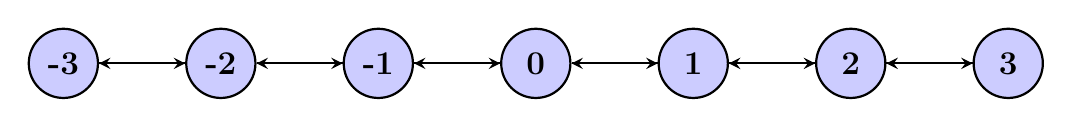
\begin{tikzpicture}[->, >=stealth, auto, thick, node distance=2cm]
    \tikzstyle{every state} = [
        fill=blue!20,
        draw=black,
        circle,
        minimum size=25pt,
        font=\large\bfseries
    ]

    \node[state] (1) at (-6, 0) {-3};
    \node[state] (2) at (-4,  0) {-2};
    \node[state] (3) at (-2,  0) {-1};
    \node[state] (4) at (0,  0) {0};
    \node[state] (5) at (2,  0) {1};
    \node[state] (6) at (4,  0) {2};
    \node[state] (7) at (6,  0) {3};

    % -3 <-> -2 <-> -1 <-> 0 <-> 1 <-> 2 <-> 3
    \path (1) edge (2); \path (2) edge (1);
    \path (2) edge (3); \path (3) edge (2);
    \path (3) edge (4); \path (4) edge (3);
    \path (4) edge (5); \path (5) edge (4);
    \path (5) edge (6); \path (6) edge (5);
    \path (6) edge (7); \path (7) edge (6);
\end{tikzpicture}
\end{center}

(a) Is $\left|X_0\right|,\left|X_1\right|,\left|X_2\right|, \ldots$ also a Markov chain? Explain. \\
Hint: For both (a) and (b), think about whether the past and future are conditionally independent given the present; don't do calculations with a 7 by 7 transition matrix!

(b) Let $\sgn$ be the sign function: $\sgn(x)=1$ if $x>0, \sgn(x)=-1$ if $x<0$, and $\sgn(0)=0$. Is $\sgn\left(X_0\right), \sgn\left(X_1\right), \sgn\left(X_2\right), \ldots$ a Markov chain? Explain.

(c) Find the stationary distribution of the chain $X_0, X_1, X_2, \ldots$.

(d) Find a simple way to modify some of the transition probabilities $q_{i,j}$ for $i \in\{-3,3\}$ to make the stationary distribution of the modified chain uniform over the states.

\solution

(a) Let $Y_n=\left|X_n\right|$. Since the chain starts at $X_0=0$, and the chain is symmetric about state $0$, we have
\begin{align*}
P(X_n=y_n) &= P(X_n=-y_n) \\
P(X_n=y_n|\left|X_n\right|=y_n) &= P(X_n=-y_n|\left|X_n\right|=y_n) = \dfrac{1}{2} \\
P(X_n=y_n|\left|X_n\right|=y_n,\ldots,\left|X_0\right|=y_0) &= P(X_n=-y_n|\left|X_n\right|=y_n,\ldots,\left|X_0\right|=y_0) = \dfrac{1}{2}
\end{align*}
Although when $y_n=0$, $-y_n=y_n$, but for a better consistency when using LOTP, we can keep this format, then we have
\begin{align*}
&\quad\ P(Y_{n+1}=y_{n+1}|Y_n=y_n,\ldots,Y_0=y_0) \\
&= P(|X_{n+1}|=y_{n+1}|\left|X_n\right|=y_n,\ldots,\left|X_0\right|=y_0) \\
&\stackrel{\text{LOTP}}{=} P(\left|X_{n+1}\right|=y_{n+1}|X_n=y_n, \left|X_n\right|=y_n,\ldots,\left|X_0\right|=y_0)P(X_n=y_n|\left|X_n\right|=y_n,\ldots,\left|X_0\right|=y_0) \\
&+ P(\left|X_{n+1}\right|=y_{n+1}|X_n=-y_n, \left|X_n\right|=y_n,\ldots,\left|X_0\right|=y_0)P(X_n=-y_n|\left|X_n\right|=y_n,\ldots,\left|X_0\right|=y_0) \\
&\stackrel{\text{symmetric}}{=} \dfrac{1}{2}\left[P(\left|X_{n+1}\right|=y_{n+1}|X_n=y_n, \left|X_n\right|=y_n,\ldots,\left|X_0\right|=y_0)+P(\left|X_{n+1}\right|=y_{n+1}|X_n=-y_n, \left|X_n\right|=y_n,\ldots,\left|X_0\right|=y_0)\right] \\
&\stackrel{\text{Markov property}}{=} \dfrac{1}{2}\left[P(\left|X_{n+1}\right|=y_{n+1}|X_n=y_n)+P(\left|X_{n+1}\right|=y_{n+1}|X_n=-y_n)\right] \\
&= P(\left|X_{n+1}\right|=y_{n+1}|X_n=y_n)P(X_n=y_n|\left|X_n\right|=y_n) + P(\left|X_{n+1}\right|=y_{n+1}|X_n=-y_n)P(X_n=-y_n|\left|X_n\right|=y_n) \\
&\stackrel{\text{LOTP}}{=} P(\left|X_{n+1}\right|=y_{n+1}|\left|X_n\right|=y_n) \\
&= P(Y_{n+1}=y_{n+1}|Y_n=y_n)
\end{align*}
So above all, $\left|X_0\right|,\left|X_1\right|,\left|X_2\right|, \ldots$ is a Markov chain.

(b) Let $Q=(q_{i,j})$ be the transition matrix, then for example
$$P(\sgn(X_{2})=1|\sgn(X_1)=1)=P(X_2\geq 1|X_1\geq 1,|X_2-X_1|=1)=q_{1,2}+q_{2,3}+q_{2,1}+q_{3,2}$$
However, if we have more information about the past, for example
$$P(\sgn(X_{2})=1|\sgn(X_1)=1,\sgn(X_0)=0)=P(X_2=2|X_1=1,X_0=0)=q_{1,2}$$
So in the we have given an example that
$$P(\sgn(X_{2})=1|\sgn(X_1)=1,\sgn(X_0)=0)\neq P(\sgn(X_{2})=1|\sgn(X_1)=1)$$
So $\sgn\left(X_0\right), \sgn\left(X_1\right), \sgn\left(X_2\right), \ldots$ is not a Markov chain.

(c) Let $Q=(q_{i,j})$ be the transition matrix, $\bpi=(\pi_i)$ be the stationary distribution, $i=-3,-2,-1,0,1,2,3$. Then we have the transition matrix is
$$Q=\begin{pmatrix}
0 & 1 & 0 & 0 & 0 & 0 & 0 \\
\frac{1}{2} & 0 & \frac{1}{2} & 0 & 0 & 0 & 0 \\
0 & \frac{1}{2} & 0 & \frac{1}{2} & 0 & 0 & 0 \\
0 & 0 & \frac{1}{2} & 0 & \frac{1}{2} & 0 & 0 \\
0 & 0 & 0 & \frac{1}{2} & 0 & \frac{1}{2} & 0 \\
0 & 0 & 0 & 0 & \frac{1}{2} & 0 & \frac{1}{2} \\
0 & 0 & 0 & 0 & 0 & 1 & 0
\end{pmatrix}$$
For the stationary distribution, we have
$$\bpi = \bpi Q \Rightarrow \begin{cases}
\pi_{-3} = \frac{1}{2}\pi_{-2} \\
\pi_{-2} = \pi_{-3} + \frac{1}{2}\pi_{-1} \\
\pi_{-1} = \frac{1}{2}\pi_{-2} + \frac{1}{2}\pi_{0} \\
\pi_{0} = \frac{1}{2}\pi_{-1} + \frac{1}{2}\pi_{1} \\
\pi_{1} = \frac{1}{2}\pi_{0} + \frac{1}{2}\pi_{2} \\
\pi_{2} = \frac{1}{2}\pi_{1} + \pi_{3} \\
\pi_{3} = \frac{1}{2}\pi_{2} \\
\sum\limits_{i=-3}^{3}\pi_i = 1
\end{cases}$$
Solve above equations, we can get the stationary distribution is
$$\bpi = \dfrac{1}{12}\left(1,2,2,2,2,2,1\right)=\left(\frac{1}{12},\frac{1}{6},\frac{1}{6},\frac{1}{6},\frac{1}{6},\frac{1}{6},\frac{1}{12}\right)$$

(d) From the theorem we have known, if $Q$ is a double stochastic matrix, then the stationary distribution is uniform. So we can modify the transition matrix $Q$ into a symmetric matrix easily. i.e. for the state $-3$, it has probability $\frac{1}{2}$ to go to $-2$ and stay at $-3$, and similarly for the state $3$. So the modified transition matrix is
$$Q'=\begin{pmatrix}
\textcolor{red}{\frac{1}{2}} & \textcolor{red}{\frac{1}{2}} & 0 & 0 & 0 & 0 & 0 \\
\frac{1}{2} & 0 & \frac{1}{2} & 0 & 0 & 0 & 0 \\
0 & \frac{1}{2} & 0 & \frac{1}{2} & 0 & 0 & 0 \\
0 & 0 & \frac{1}{2} & 0 & \frac{1}{2} & 0 & 0 \\
0 & 0 & 0 & \frac{1}{2} & 0 & \frac{1}{2} & 0 \\
0 & 0 & 0 & 0 & \frac{1}{2} & 0 & \frac{1}{2} \\
0 & 0 & 0 & 0 & 0 & \textcolor{red}{\frac{1}{2}} & \textcolor{red}{\frac{1}{2}}
\end{pmatrix}$$
Then the stationary distribution of the modified chain is uniform over the states.

\end{homeworkProblem}

\newpage
\begin{homeworkProblem}

\textbf{Beta Normal Distribution:} generate samples from the beta distribution $\Beta(5,5)$

(a) Implement a Metropolis-Hastings algorithm.

(b) Implement a Hamiltonian Monte Carlo algorithm.

(c) Implement with the Acceptance-Rejection Method.

(d) Compare the above three algorithms with corresponding pros and cons.

\solution

Let $X\sim \Beta(5,5)$. We can calculate the beta integral:
$$\beta(5,5)=\dfrac{\Gamma(5)\cdot\Gamma(5)}{\Gamma(10)}=\dfrac{4!\cdot 4!}{9!}=\dfrac{1}{630}$$
Then we can calculate the PDF of $X$:
$$f(x)=f_X(x)=\dfrac{1}{\beta(5,5)}x^{5-1}(1-x)^{5-1}=630x^4(1-x)^4 ,0<x<1$$

(a) Since the support of Beta distributio is $[0,1]$, so we can choose the proposal distribution to be $\Unif(1)$, which means that the one-step transition probability density from state $x$ to $y$ is $f_{x,y}=1$, thus we can get that the acceptance rate:
$$a_{x,y}=\min\left(\dfrac{\pi_jf_{j,i}}{\pi_if_{i,j}},1\right)=\min\left(\dfrac{j^4(1-j)^4}{i^4(1-i)^4},1\right)$$
Then we can do the Discrete time continuous state Metropolis-Hastings algorithm to sample the distribution $\Beta(5,5)$ in 1000000 samples, and the burn in is set to be 10000 samples. The result is as follows:
\begin{figure}[h]
    \centering
    \includegraphics[width=0.5\textwidth]{./figure/p5/MH.png}
\end{figure}

(b) Since $\pi_x$ is a the stationary distribution $\Beta(5,5)$, and we can ignore the constant form, so the potential energy is
$$U(x)=-\log(\pi_x) = -\log(630) -4\log(x(1-x)) \stackrel{\text{ignore const}}{\Rightarrow} U(x)=-4\log(x(1-x))$$
And let the mass be 1, then the Kinetic energy is
$$V(\omega)=\dfrac{1}{2}\omega^2, \quad\text{where } \omega\sim\N(0,1)$$
Thus the Hamiltonian energy is
$$H(x,\omega)=U(x)+V(\omega)=-4\log(x(1-x))+\dfrac{1}{2}\omega^2$$
Initially, set $x_0=0.5, \omega_0\sim\N(0,1)$, apply the Leapfrog method to sample:
\begin{align*}
\omega_{t+\frac{\delta}{2}} &= \omega_t - \frac{\delta}{2}\cdot \dfrac{\dU(x_t)}{\dx_t} = \omega_t - \frac{\delta}{2}\cdot \left(-\dfrac{4}{x_t}+\dfrac{4}{1-x_t}\right) \\
x_{t+\delta} &= x_t + \delta \cdot \dfrac{\dV(\omega_{t+\frac{\delta}{2}})}{\domega_{t+\frac{\delta}{2}}} = x_t + \delta\cdot \omega_{t+\frac{\delta}{2}} \\
\omega_{t+\delta} &= \omega_{t+\frac{\delta}{2}} - \frac{\delta}{2}\cdot \dfrac{\dU(x_{t+\delta})}{\dx_{t+\delta}} = \omega_{t+\frac{\delta}{2}} - \frac{\delta}{2}\cdot \left(-\dfrac{4}{x_{t+\delta}}+\dfrac{4}{1-x_{t+\delta}}\right)
\end{align*}
Due to the range limitation of $x\in(0,1)$, we can add a reflection bound at $x=0$ and $x=1$, i.e. when applying Leapfrog, if $x<0$, then set $x\gets -x, \omega\gets -\omega$, if $x>1$, then set $x\gets 2-x, \omega\gets -\omega$. After Leapfrog $L$ steps, we can get the state $(x_L, \omega_L)$. And set $(x_L, -\omega_L)$ to be the proposal distribution. And the accept rate for the Hamiltonian Monte Carlo algorithm is
$$a_{(x_0,\omega_0),(x_L,-\omega_L)}=\min\left(\dfrac{\exp\left(-H(x_L,-\omega_L)\right)}{\exp\left(-H(x_0,\omega_0)\right)}, 1\right)=\min\left(\dfrac{\exp\left(-U(x_L)-V(-\omega_L)\right)}{\exp\left(-U(x_0)-V(\omega_0)\right)}, 1\right)$$
We step the stepsize to be $\delta=0.05, L=15$, additionally, since the support is $(0,1)$, so for numerical accuracy, we clip x into the range $[10^{-10},1-10^{-10}]$. One trajectory and sample results are as follows:
\begin{figure}[h]
    \centering
    \includegraphics[width=0.5\textwidth]{./figure/p5/trajectory.png}
    \includegraphics[width=0.5\textwidth]{./figure/p5/Hamiltonian.png}
\end{figure}

(c) As for the acceptance-rejection algorithm, since the support of Beta distribution is $(0,1)$, so we can take $Y\sim \Unif(0,1)$. And its PDF is $g(y)=f_Y(y)=1$. \\
Let $c$ donate a constant:
$$c = \sup_y\dfrac{f(y)}{g(y)} = \sup_y\dfrac{20y(1-y)^3}{1}=630x^4(1-x)^4\big|_{y=\frac{1}{2}}=\dfrac{315}{128}$$
Then we can apply the Acceptance-Rejection algorithm to generate the samples on $X\sim \Beta(5,5)$:
\begin{figure}[h]
    \centering
    \includegraphics[width=0.5\textwidth]{./figure/p5/accept_reject.png}
\end{figure}

(d) 1. Metropolis-Hastings Algorithm: \\
Advantages: It is highly general-purpose, could applicable to a wide variety of distributions, and it does not require the normalization constant of the target distribution. \\
Disadvantages: Samples are often requires select a suitable distribution, and requires steps to burn up.

2. Hamiltonian Monte Carlo Algorithm: \\
Advantages: Due to the conservation of energy, the acceptance rate should be $1$. But there exists numerical error, however quite close to $1$, which means it has quite high acceptance rate. The samples are efficient, especially in high-dimensional problems. \\
Disadvantages: Requires computation of gradients, increasing implementation complexity. Sensitive to parameters: step size $\delta$ and number of steps for LeapFrog $L$.

3. Acceptance-Rejection Method: \\
Advantages: It produces independent samples, and is simple to implement. If the good envelope function is suitable, it is efficient. \\
Disadvantages: Efficiency depends heavily on the choice of proposal distribution, for example, ours implement has a quite low acceptance rate, which is only 0.0038838.

\end{homeworkProblem}

\newpage
\begin{homeworkProblem}

\textbf{Approximating the Optimal Value Function}

Consider a finite MDP $M=\langle \mS, \A, T, \R, \gamma\rangle$, where $\mS$ is the state space, $\A$ action space, $T$ transition probabilities, $\R$ reward function and $\gamma$ the discount factor. Define $Q^*$ to be the optimal state-action value $Q^*(s, a)=Q_{\pi^*}(s, a)$ where $\pi^*$ is the optimal policy. Assume we have an estimate $\tilde{Q}$ of $Q^*$, and $\tilde{Q}$ is bounded by $L_{\infty}$ norm as follows:
$$\|\tilde{Q}-Q^*\|_{\infty} \leq \epsilon$$
Where $\|x\|_{\infty}=\max\limits_{s, a}|x(s, a)|$. \\
Assume that we are following the greedy policy with respect to $\tilde{Q}, \pi(s)=\argmax\limits_{a \in \A} \tilde{Q}(s, a)$. We want to show that the following holds:
$$V_\pi(s) \geq V^*(s)-\frac{2 \epsilon}{1-\gamma}$$
Where $V_{\pi}(s)$ is the value function of the greedy policy $\pi$ and $V^*(s)=\max\limits_{a \in \A} Q^*(s, a)$ is the optimal value function. This shows that if we compute an approximately optimal state-action value function and then extract the greedy policy for that approximate state-action value function, the resulting policy still does well in the real MDP.

(a) Let $\pi^*$ be the optimal policy, $V^*$ the optimal value function and as defined above $\pi(s)=\argmax\limits_{a \in \A} \tilde{Q}(s, a)$. Show the following bound holds for all states $s \in \mS$.
$$V^*(s)-Q^*(s, \pi(s)) \leq 2 \epsilon$$

(b) Using the results of part 1, prove that $V_\pi(s) \geq V^*(s)-\frac{2\epsilon}{1-\gamma}$. \\
Now we show that this bound is tight. Consider the 2-state MDP illustrated in Figure \ref{fig:approximate}. State $s_1$ has two actions, ``\textit{stay}" self transition with reward 0 and ``\textit{go}" that goes
to state $s_2$ with reward $2\epsilon$. State $s_2$ transitions to itself with reward $2\epsilon$ for every time step afterwards.
\begin{figure}[h]
    \centering
    \vspace{-0.4cm}
    \includegraphics[width=0.5\textwidth]{./figure/approximate.png}
    \vspace{-0.4cm}
    \caption{A 2-state MDP.}
    \vspace{-0.4cm}
    \label{fig:approximate}
\end{figure}

(c) Compute the optimal value function $V^*(s)$ for each state and the optimal stateaction value function $Q^*(s, a)$ for state $s_1$ and each action.

(d) Show that there exists an approximate state-action value function $\tilde{Q}$ with $\epsilon$ error (measured with $L_{\infty}$ norm), such that $V_\pi\left(s_1\right)-V^*\left(s_1\right)=-\frac{2 \epsilon}{1-\gamma}$, where $\pi(s)=$ $\argmax\limits_{a \in \A} \tilde{Q}(s, a)$. (You may need to define a consistent tie break rule)

\solution

(a) Since $\pi(s)$ is the optimal policy for $\tilde{Q}$, thus it has $\tilde{Q}(s, \pi(s)) \geq \tilde{Q}(s, \pi^*(s))$, so
\begin{align*}
V^*(s)-Q^*(s,\pi(s)) &= V^*(s)-\tilde{Q}(s,\pi(s))+\tilde{Q}(s,\pi(s))-Q^*(s,\pi(s)) \\
\text{(Since $\|\tilde{Q}-Q^*\|_{\infty} \leq \epsilon$)}\quad & \leq V^*(s) - \tilde{Q}(s, \pi(s)) + \epsilon \\
\text{(Since $\tilde{Q}(s, \pi(s)) \geq \tilde{Q}(s, \pi^*(s))$)}\quad & \leq V^*(s) - \tilde{Q}(s, \pi^*(s)) + \epsilon \\
&= Q^*(s, \pi^*(s)) - \tilde{Q}(s, \pi^*(s)) + \epsilon \\
\text{(Since $\|\tilde{Q}-Q^*\|_{\infty}\leq \epsilon$)}\quad & \leq 2\epsilon
\end{align*}
So above all, we have proved that $V^*(s) - Q^*(s, \pi(s)) \leq 2\epsilon$.

(b) Using Bellman Exceptation Equation, we have
\begin{align*}
Q^*(s, a) &= \R_s^{a} + \gamma\sum_{s'\in\mS}\mP_{s,s'}^aV^*(s') \\
\tilde{Q}(s, a) &= \R_s^{a} + \gamma\sum_{s'\in\mS}\mP_{s,s'}^aV_{\pi}(s')
\end{align*}
Combining them, we can get that
\begin{align*}
V^*(s) - V_{\pi}(s) &= V^*(s) - Q^*(s, \pi(s)) + Q^*(s, \pi(s)) - V_{\pi}(s) \\
\text{(Conclusion of (a))}\quad &\leq 2\epsilon + Q^*(s, \pi(s)) - Q(s, \pi(s)) \\
&= 2\epsilon + \left(\R_{s}^{\pi(s)} + \gamma\sum_{s'\in\mS}\mP_{\pi(s),s'}^aV^*(s')\right) - \left(\R_{s}^{\pi(s)} + \gamma\sum_{s'\in\mS}\mP_{\pi(s),s'}^aV_{\pi}(s')\right) \\
&= 2\epsilon + \gamma\sum_{s'\in\mS}\mP_{\pi(s),s'}^a\left(V^*(s') - V_{\pi}(s')\right)
\end{align*}
Suppose that the upper bound of $V*(s)-V_{\pi}(s)$ is $U$, i.e. $\forall s \in \mS, V^*(s)-V_{\pi}(s) \leq U$, thus we have:
\begin{align*}
\forall s \in \mS,\quad V^*(s) - V_{\pi}(s) &\leq 2\epsilon + \gamma U \\
\Rightarrow \qquad\qquad\qquad\quad U &\leq 2\epsilon + \gamma U \\
\Rightarrow \qquad\qquad (1-\gamma)U &\leq 2\epsilon \\
\Rightarrow \qquad\qquad\qquad\quad U &\leq \dfrac{2\epsilon}{1-\gamma}
\end{align*}
So above all, we have proved:
$$V^*(s) - V_{\pi}(s)\leq \dfrac{2\epsilon}{1-\gamma} \Rightarrow V_{\pi}(s) \geq V^*(s) - \dfrac{2\epsilon}{1-\gamma}$$

(c) It is obvious that the optimal policy is $\pi_*(s_1)=\text{go}$, from the Bellman Optimility Equation, we have
\begin{align*}
V^*(s_2) &= 2\epsilon + \gamma V^*(s_2) \Rightarrow V^*(s_2) = \frac{2\epsilon}{1-\gamma} \\
V^*(s_1) &= V^{\pi_*}(s_1) = 2\epsilon + \gamma V^*(s_2) \Rightarrow V^*(s_1) = \frac{2\epsilon}{1-\gamma} \\
Q^*(s_1, \text{go}) &= 2\epsilon + \gamma V^*(s_2) \Rightarrow Q^*(s_1, \text{go}) = \frac{2\epsilon}{1-\gamma} \\
Q^*(s_1, \text{stay}) &= 0 + \gamma V^*(s_1) \Rightarrow Q^*(s_1, \text{stay}) = \frac{2\epsilon\gamma}{1-\gamma}
\end{align*}

(d) Since the approximate state-action value function allowed the $\epsilon$ error, and we could observe that the difference between $Q^*(s_1,\text{go})$ and $Q^*(s_1,\text{stay})$ is $\dfrac{2\epsilon}{1-\gamma} - \dfrac{2\epsilon\gamma}{1-\gamma} = 2\epsilon$. Thus we can set $\tilde{Q}$ to be
\begin{align*}
\tilde{Q}(s_1, \text{go}) = Q^*(s_1, \text{go}) - \epsilon &\Rightarrow \tilde{Q}(s_1,\text{go}) = \frac{\epsilon(1+\gamma)}{1-\gamma} \\
\tilde{Q}(s_1, \text{stay}) = Q^*(s_1, \text{stay}) + \epsilon &\Rightarrow \tilde{Q}(s_1,\text{stay}) = \frac{\epsilon(1+\gamma)}{1-\gamma}
\end{align*}
Since the estimated $\tilde{Q}$ for state $s_1$ and its two actions are tie, so we can define the policy for tie: $\pi(\text{stay}|s_1)=1$. Thus $V_{\pi}(s_1)=0 + \gamma V_{\pi}(s_1)\Rightarrow V_{\pi}(s_1)=0$.
Since $V^*(s_1)=\dfrac{2\epsilon}{1-\gamma}$, thus $V_{\pi}(s_1)-V^*(s_1)=-\dfrac{2\epsilon}{1-\gamma}$.

So above all, we have proved that the $V_{\pi}(s)\geq V^*(s)-\dfrac{2\epsilon}{1-\gamma}$ is a tight bound.

\end{homeworkProblem}

\newpage
\begin{homeworkProblem}

\textbf{Bivariate Standard Normal Distribution:} Implement a Gibbs sampler to generate samples from a bivariate standard normal distribution with correlation $\rho=0.6,-0.6$.

\solution

Suppose that the correlation of the bivariate standard normal distribution is $\rho\in(-1,1)$, which means that the covariance matrix is $\Sigma=\begin{bmatrix}
    1 & \rho \\
    \rho & 1
\end{bmatrix}$. Thus the joint PDF is
$$f_{X,Y}(x,y)=\dfrac{1}{2\pi\sqrt{1-\rho^2}}e^{-\frac{x^2-2\rho xy+y^2}{2(1-\rho^2)}}$$
So we can derive that the conditional PDF of $X$ given $Y=y$ is
$$f_{X|Y=y}(x|Y=y)\propto e^{-\frac{(x-\rho y)^2}{2(1-\rho^2)}}\sim\N(\rho y,1-\rho^2)$$
Similarly, the conditional PDF of $Y$ given $X=x$ is
$$f_{Y|X=x}(y|X=x)\propto e^{-\frac{(y-\rho x)^2}{2(1-\rho^2)}}\sim\N(\rho x,1-\rho^2)$$
Then we can apply the Gibbs sampler to generate samples from the bivariate standard normal distribution with correlation $\rho=0.6,-0.6$ in 1000000 samples, and the burn in is set to be 10000 samples. The results are as follows:

\begin{figure}[h]
    \centering
    \includegraphics[width=0.48\textwidth]{./figure/p7/-0.6.png}
    \includegraphics[width=0.48\textwidth]{./figure/p7/0.6.png}
\end{figure}

\end{homeworkProblem}

\newpage
\begin{homeworkProblem}

\textbf{Chicken-Egg with Unknown Parameters:} The parameter setting: $\lambda=10, a=b=1, x=7$.

(a) Implement a Gibbs sampler to find the posterior mean and the variance of $p$ after observing $x$ hatched eggs.

(b) Implement a Metropolis-Hastings algorithm to find the posterior mean and variance of $p$ after observing $x$ hatched eggs.

(c) Compare such two methods of MCMC.

\solution

Let $N\sim\Pois(\lambda)$ donates number of eggs. \\
The prior distribution of the hatch probability is $P\sim\Beta(a,b)$. \\
$X|P=p\sim\Pois(\lambda p)$ is the number of hatched eggs, $N-X|P=p\sim\Pois(\lambda(1-p))$ is the number of unhatched eggs.

(a) Directly sample the conditional probability above is complex, so we consider the conditional joint distribution of $X,N|P$: \\
Since $X|N=n,P=p\sim\Bin(n,p)$, and we have the prior $P\sim\Beta(a,b)$, from the Beta-Binomial conjugate, we can get that
$$P|N=n,X=x\sim\Beta(a+x,b+n-x)$$
And from the definition of $N$ and $X$, we have
$$f_{N|P,X}(n|P=p,X=x) \sim x + \Pois(\lambda(1-p))$$
The conditional distributions are all easy to sample, so we can use the Gibbs sampling to sample the joint distribution of $P,N|X$, then the marginal distribution of $P|X=x$ and $N|X=x$ can be calculated. Set the initial state to be $p_0=0.5, n_0=7$.  The sampling results are as follows:
\begin{figure}[h]
    \centering
    \includegraphics[width=0.49\textwidth]{./figure/p8/Gibbs_P.png}
    \includegraphics[width=0.49\textwidth]{./figure/p8/Gibbs_N.png}
\end{figure}

The estimated P given $X = 7$ has mean: $0.68449$, variance: $0.03196$.

(b) Directly calculate the posterior distribution of $P$ with Metropolis-Hastings algorithm:
\begin{align*}
f_{P|X}(p|X=x) &\propto P(X=x|P=p)f_P(p) \\
&= e^{-(\lambda p)}\dfrac{(\lambda p)^x}{x!} \cdot \dfrac{1}{\beta(a,b)}p^{a-1}(1-p)^{b-1} \\
&\propto e^{-\lambda p}(\lambda p)^x\cdot p^{a-1}(1-p)^{b-1}
\end{align*}
Since the support of $P$ is $[0,1]$, thus we can $\Unif(0,1)$ to be the proposal distribution, i.e. the one-step transition probability density from state $x$ to $y$ is $f_{i,j}=f_{X_{n+1}|X_n}(j|i)=1,j>0$, so we can get that the acceptance rate:
$$a_{i,j}=\min\left(\dfrac{\pi_jf_{j,i}}{\pi_if_{i,j}},1\right)=\min\left(\dfrac{e^{-\lambda j}(\lambda j)^x\cdot j^{a-1}(1-j)^{b-1}}{e^{-\lambda i}(\lambda i)^x\cdot i^{a-1}(1-i)^{b-1}},1\right)$$
The sampling results are as follows:
\begin{figure}[h]
    \centering
    \includegraphics[width=0.6\textwidth]{./figure/p8/MH_P.png}
\end{figure}
The estimated P given $X = 7$ has mean: $0.68468$, variance: $0.03198$.

(c) We can see that both Gibbs sampling and Metropolis-Hastings algorithm with same sample number as burn in number have a similar estimation.

Metropolis-Hastings: \\
Advantages: It can sample many different distributions with suitable proposal distribution, without requiring the conditional distribution is easy to sample. \\
Disadvantages: It is actually a accept-reject method, if the simulation steps are not enough, it may reject many times and stay at the same state, also, it may need more calculations.


Gibbs sampling:
Advantages: It need less calculations, do not need to reject samples, thus it is efficient. \\
Disadvantages: It need to sample the conditional distribution, which required to be easy to sample. If the conditional distributions are complex, it still require Metropolis-Hastings algorithm or other sampling methods to generate a single sample, which is not efficient.

\end{homeworkProblem}

\newpage
\begin{homeworkProblem}
Uniform is the only distribution that takes the maximum entropy.

\textcolor{blue}{Solution} \\

Consider the diecrete case $|\mathcal{X}|<\infty$. \\

1. Consider the KL-divergence $D\left(p(x)\|q(x)\right)\geq 0$.\\
proof:
\begin{align*}
-D\left(p(x)\|q(x)\right) &= \sum_{x}p(x)\log\dfrac{q(x)}{p(x)} \\
&= \mathbb{E}_{x\sim p(x)}\left[\log\dfrac{q(x)}{p(x)}\right] \\
&\leq \log\mathbb{E}_{x\sim p(x)}\left[\dfrac{q(x)}{p(x)}\right] \text{\ \ \ \ (Jensen's Inequality)} \\
&= \log\sum_{x}p(x)\dfrac{q(x)}{p(x)} \\
&= 0
\end{align*}
i.e. $D\left(p(x)\|q(x)\right)\geq 0$. \\
If and only if when $p(x)=q(x)$, the equality holds, this is because Jensen's Inequality holds when the function is linear.

2. Consider the entropy $H(X)=\E\left[-\log p(x)\right]=\sum_{x\in\mathcal{X}}p(x)\log\dfrac{1}{p(x)}$. \\
Let $u(x)=\dfrac{1}{|\mathcal{X}|}$, then
\begin{align*}
D\left(p\|u\right) &= \sum_{x\in\mathcal{X}}p(x)\log\dfrac{p(x)}{u(x)} \\
&= \sum_{x\in\mathcal{X}}p(x)\log|\mathcal{X}| - \sum_{x\in\mathcal{X}}p(x)\log\dfrac{1}{p(x)} \\
&= \log|\mathcal{X}| - H(X) \\
&\geq 0
\end{align*}
If and only if $p(x)=u(x)$, the equality holds, i.e. $H(X)$ takes the maximum value $\log|\mathcal{X}|$.

So above all, the uniform distribution is the only distribution that takes the maximum entropy if $|\mathcal{X}|<\infty$.

\end{homeworkProblem}

\end{document}